
This section introduces the HPC application studied in this research and delves into characterizing them. The main source of these applications is the ongoing Exascale Proxy Application Project~\cite{ecpapp}, commonly known as ECP proxy apps. Along with these proxy apps, Lulesh~\cite{karlin2012lulesh}, another commonly used mini-app in the HPC community, is considered in this study. For characterisation, at first, hostspot analysis is performed using Intel Vtune(2022.3.0) to identify the functions with high execution time. Then, Intel Advisor is used to generate Roofline models to identify the compute-memory intensity of those functions. Table~\ref{table:apps} shows the application names along with the functions and Figure~\ref{fig:roofline} shows the position in the Roofline model. All the functions studied in this research are memory intensive.

\begin{figure}[t]%[bp]
\begin{center}
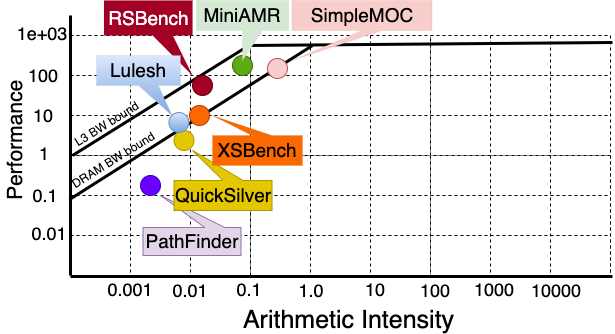
\includegraphics[width=1\linewidth]{MEMSYS22/figures/roofline/roofline_pim.png}
\end{center}
  \vspace{-0.1in}
%\caption{Approximate Roofline positioning of the studied functions of different applications.}
\caption{Approximate representation of HPC application kernels on the roofline model.}
\label{fig:roofline}
\vspace{-0.2in}
\end{figure}



\subsection{SimpleMOC}
SimpleMOC mini-app is designed to demonstrate the performance and viability of the Method of Characteristics (MOC) for 3D neutron transport calculations for full scale
light water reactor simulation. In this application, $attenuate\_fluxes$ function is one of the major contributor in execution time and is bound by DRAM Bandwidth (see Figure~\ref{fig:roofline}). 


%./PathFinder.x -x ../data/scaleData/1kx750.adj_list
\subsection{PathFinder}
PathFinder is implemented for searching signatures in directed and cyclic graphs. It searches the path between signatures and lables in the graph. One of the main functions in PathFinder is $findAndRecordAllPaths$, which is DRAM bandwidth bound and has the lowest arithmetic intensity of all the functions studied in this research. 

\subsection{XSBench}
XSBench represents a key computational kernel of the Monte Carlo neutron transport algorithm, which performs continuous energy macroscopic neutron cross section lookup. The hotspot and Roofline analysis identify $calculate\_micro\_xs$ function as one of the major memory bound functions. 

\subsection{RSBench}
Similar to XSBench, RSBench also represents a kernel for Monte Carlo neutron transport algorithm. It represents the multipole method for performing continuous energy macroscopic neutron cross section lookups. The hotspot and Roofline analysis reveals $c\_mul$ function as one of the major memory bound function.


\subsection{MiniAMR}
MiniAMR performs adaptive mesh refinement which divides a unit cube computational domain and applies stencil calculation. The blocks have equal number for cell distribution and communicates to their neighbors using ghost values. As expected, the $stencil\_calc$ function is the main memory bound function for this application which is bound by level 3 cache bandwidth (see Figure~\ref{fig:roofline}). 

%./qs --nParticles=10000
\subsection{Quicksilver}
Quicksilver solves a simplified dynamic monte carlo particle transport problem to partially implement the Mercury workload. It replicates the memory access pattern, communication and branching of Mercury for problems using multi-group cross sections. The function $macroscopicCrossSection$ is found to be the one of the hotspots, which is a memory intensive kernel bound by DRAM bandwidth in the Roofline model.

\subsection{Lulesh}
Lulesh (Livermore Unstructured Lagrangian Explicit Shock Hydrodynamics) is a well-known HPC proxy-app developed in Lawrence Livermore National Laboratory. This application exhibits different memory access patterns for a 3D mesh data structure where more than twenty functions are identified as memory bound~\cite{monil2022mapredict}, which makes it a feasible candidate for PIM study. In this study, we consider the function $CalcKinematicsForElems$ for evaluation.
%Two functions in Lulesh is in our interest. 1). CalcFBHourglassForce (highest time consuming but hihger AI) and 2). CalcElemCharacteristicLength (yellow but lowest AI)
%CalcKinematicsForElems




%
%
\begin{table}[t]
%\normalsize
\small
\caption{HPC Benchmarks and their Memory-Bound/Critical Kernel/Functions identified}
\centering
%    \begin{tabularx}{\columnwidth}{lcc}
    \begin{tabularx}{\columnwidth}{ccc}
    %\begin{tabularx}{7.2cm}{lcc}
\toprule
    % \hline
    Bechmarks & Function & Memory/compute bound \\
\midrule
%jacobi & - & +++ \\
%laplace  & - & +++ \\

%Lulesh-2 & CalcElemCharacteristicLength & DRAM BW bound \\
SimpleMOC & attenuate\_fluxes & Main Memory BW bound \\
PathFinder   & findAndRecordAllPaths & Main Memory BW bound \\
XSBench      & calculate\_micro\_xs & Main Memory BW bound \\
RSBench      & c\_mul & L3 BW bound \\
MiniAMR      & stencil\_calc & L3 BW bound \\
QuickSilver      & macroscopicCrossSection & Main Memory BW bound \\
Lulesh & CalcKinematicsForElems & Main Memory BW bound \\
\bottomrule
   \end{tabularx}
\label{table:apps}
%\vspace{-0.5cm}
\end{table}
%
%
%
%\begin{figure}[t!]
%\centering
%\includegraphics[width=\columnwidth]{figure/processor.png}
%\caption{Schematic view of the Next Generation Microprocessor~(NGMP)}
%\label{fig:processor}
%%\vspace{-0.4cm}
%\end{figure}



%-	Roofline model \\
%-	Identifying functions that are memory intensive \\


%\subsection{Jacobi}
%The main function in Jacobi is the $stencil\_jacobi$ function which is a memory bound kernel (see Fig.~\ref{fig:roof-jacobi}). 







%\begin{figure}[t!]
%\centering
%\includegraphics[width=70mm, height= 50mm]{figure/pmtj.pdf}
%%\vspace{.5em} 
%\caption{STT-MRAM cell}
%%\vspace{-1.5em} 
%\label{fig:pmtj}
%%\vspace{-0.3cm}   
%\end{figure} 
%
%
%
%
%  
%\looseness -1
%
%
%
%\begin{figure}[t!]
%\centering
%\includegraphics[width=\columnwidth]{figure/DeviceCapacity.pdf}
%%\vspace{.5em} 
%\caption{DRAM and STT-MRAM capacity growth in years} %\pr{23-Feb: Kazi, do we have any data from after 2016? Take care of this only if you have some extra time. }}
%%\vspace{-1.5em} 
%\label{fig:Capa}
%\vspace{-0.3cm}  
%\end{figure}  


%\begin{figure}[t]%[bp]
%\begin{center}
%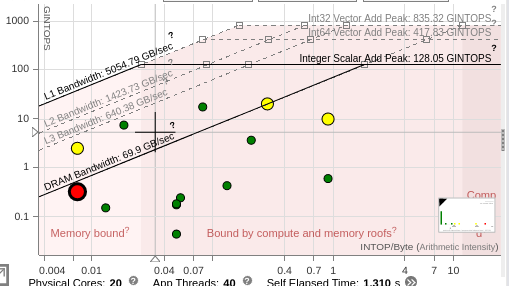
\includegraphics[width=1\linewidth]{MEMSYS22/figures/roofline/pathfinder.png}
%\end{center}
%  \vspace{-0.1in}
%\caption{Positioning of the main compute kernel of PathFinder app in Roofline. Here the red circle indicates the $findAndRecordAllPaths$ function }
%\label{fig:roof-pathfinder}
%\vspace{-0.2in}
%\end{figure}

%\begin{figure}[t]%[bp]
%\begin{center}
%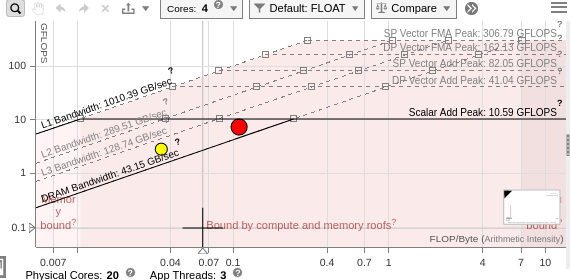
\includegraphics[width=1\linewidth]{MEMSYS22/figures/roofline/miniamr.png}
%\end{center}
%  \vspace{-0.1in}
%\caption{Positioning of the main compute kernel of MiniAMR app in Roofline. Here the red circle indicates the $stencil\_calc$ function }
%\label{fig:roof-miniamr}
%\vspace{-0.2in}
%\end{figure}



%\begin{figure}[h]%[bp]
%\begin{center}
%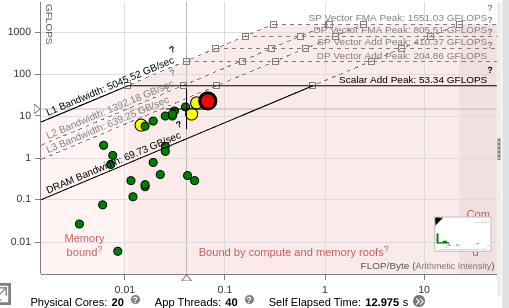
\includegraphics[width=1\linewidth]{MEMSYS22/figures/roofline/simplesoc.png}
%\end{center}
%  \vspace{-0.1in}
%\caption{Positioning of the main compute kernel of SimpleMOC app in Roofline. Here the red circle indicates the $attenuate\_fluxes$ function }
%\label{fig:roof-simplemoc}
%\vspace{-0.2in}
%\end{figure}